%% abtex2-modelo-projeto-pesquisa.tex, v-1.9.6 laurocesar
%% Copyright 2012-2016 by abnTeX2 group at http://www.abntex.net.br/ 
%%
%% This work may be distributed and/or modified under the
%% conditions of the LaTeX Project Public License, either version 1.3
%% of this license or (at your option) any later version.
%% The latest version of this license is in
%%   http://www.latex-project.org/lppl.txt
%% and version 1.3 or later is part of all distributions of LaTeX
%% version 2005/12/01 or later.
%%
%% This work has the LPPL maintenance status `maintained'.
%% 
%% The Current Maintainer of this work is the abnTeX2 team, led
%% by Lauro César Araujo. Further information are available on 
%% http://www.abntex.net.br/
%%
%% This work consists of the files abntex2-modelo-projeto-pesquisa.tex
%% and abntex2-modelo-references.bib
%%

% ------------------------------------------------------------------------
% ------------------------------------------------------------------------
% abnTeX2: Modelo de Projeto de pesquisa em conformidade com 
% ABNT NBR 15287:2011 Informação e documentação - Projeto de pesquisa -
% Apresentação 
% ------------------------------------------------------------------------ 
% ------------------------------------------------------------------------

\documentclass[
% -- opções da classe memoir --
article,			% indica que é um artigo acadêmico
12pt,				% tamanho da fonte
openright,			% capítulos começam em pág ímpar (insere página vazia caso preciso)
oneside,			% para impressão em recto. Oposto a twoside
%twoside,			% para impressão em recto e verso. Oposto a oneside
a4paper,			% tamanho do papel. 
% -- opções da classe abntex2 --
chapter=TITLE,		% títulos de capítulos convertidos em letras maiúsculas
section=TITLE,		% títulos de seções convertidos em letras maiúsculas
subsection=TITLE,	% títulos de subseções convertidos em letras maiúsculas
subsubsection=TITLE,% títulos de subsubseções convertidos em letras maiúsculas
subsubsubsection=TITLE, % títulos de subsubsubseções em letras maiúsculas
% -- opções do pacote babel --
english,			% idioma adicional para hifenização
%french,			% idioma adicional para hifenização
%spanish,			% idioma adicional para hifenização
brazil,				% o último idioma é o principal do documento
]{abntex2}

% ---
% PACOTES
% ---

% ---
% Pacotes fundamentais 
% ---
\usepackage{lmodern}			% Usa a fonte Latin Modern
\usepackage[T1]{fontenc}		% Selecao de codigos de fonte.
\usepackage[utf8]{inputenc}		% Codificacao do documento (conversão automática dos acentos)
\usepackage{indentfirst}		% Indenta o primeiro parágrafo de cada seção.
\usepackage{color}				% Controle das cores
\usepackage{graphicx}			% Inclusão de gráficos
\usepackage{microtype} 			% para melhorias de justificação
%\usepackage[none]{hyphenat} 			% Desativa ifenização
\usepackage{booktabs}
\usepackage[svgnames,table]{xcolor}
\usepackage[tableposition=above]{caption}
\usepackage{tabularx}
\usepackage{float}              % float H para imagens e tabelas
% ---

% ---
% Pacotes adicionais, usados apenas no âmbito do Modelo Canônico do abnteX2
% ---
\usepackage{lipsum}				% para geração de dummy text
% ---

% ---
% Pacotes de citações
% ---
\usepackage[brazilian,hyperpageref]{backref}	 % Paginas com as citações na bibl
\usepackage[alf]{abntex2cite}	% Citações padrão ABNT

% --- 
% CONFIGURAÇÕES DE PACOTES
% --- 

% ---
% Configurações do pacote backref
% Usado sem a opção hyperpageref de backref
\renewcommand{\backrefpagesname}{Citado na(s) página(s):~}
% Texto padrão antes do número das páginas
\renewcommand{\backref}{}
% Define os textos da citação
\renewcommand*{\backrefalt}[4]{%
    \ifcase #1 %
        Nenhuma citação no texto.%
        \or
        Citado na página #2.%
    \else
        Citado #1 vezes nas páginas #2.%
\fi}%
% ---

% ---
% Configurações do modelo IFPR
\usepackage{abntex2ifpr}

% ---
% Informações de dados para CAPA, FOLHA DE ROSTO e FOLHA DE APROVAÇÃO
% ---
\titulo{Automatização de Mineração de Criptomoedas Com Distribuição
Linux}
\autor{Mateus Mercer}
\local{Londrina}
\data{2018}
\orientador{Prof\@. Dr\@. Rodolfo Barriviera}
%\coorientador{INSIRA O COORIENTADOR}
\convidadoum{INSIRA O CONVIDADO 1}
\convidadodois{INSIRA O CONVIDADO 2}
\curso{Curso Superior de Tecnologia em Análise e Desenvolvimento de Sistemas}
% O preambulo deve conter o tipo do trabalho, o objetivo, 
% o nome da instituição e a área de concentração 
\preambulo{Trabalho de Conclusão de Curso apresentado ao \imprimircurso do Instituto 
    Federal do Paraná \@\textendash\@ Campus Londrina, como 
requisito parcial de avaliação.}
% ---

% ---
% Configurações de aparência do PDF final

% alterando o aspecto da cor azul
\definecolor{blue}{RGB}{41,5,195}

% Ajude o professor na hora da correção com duplo espaçamento
%\linespread{2}

% informações do PDF
\makeatletter
\hypersetup{%
    %pagebackref=true,
    pdftitle={\@title}, 
    pdfauthor={\@author},
    pdfsubject={\imprimirpreambulo},
    pdfcreator={LaTeX with abnTeX2},
    pdfkeywords={abnt}{latex}{abntex}{abntex2}{projeto de pesquisa}, 
    colorlinks=false,       		% false: boxed links; true: colored links
    linkcolor=blue,          	% color of internal links
    citecolor=blue,        		% color of links to bibliography
    filecolor=magenta,      		% color of file links
    urlcolor=blue,
    bookmarksdepth=4
}
\makeatother
% --- 

% --- 
% Espaçamentos entre linhas e parágrafos 
% --- 

% O tamanho do parágrafo é dado por:
\setlength{\parindent}{1.3cm}

% Controle do espaçamento entre um parágrafo e outro:
\setlength{\parskip}{0.2cm}  % tente também \onelineskip

% ---
% compila o indice
% ---
\makeindex
% ---

% ---
% Aonde as imagens estao
% ---
\graphicspath{{imagens/}}
% ---

% ---
% Facilidade em inserir código
% ---
\def\code#1{\texttt{#1}}

% ----
% Início do documento
% ----
\begin{document}

% Seleciona o idioma do documento (conforme pacotes do babel)
%\selectlanguage{english}
\selectlanguage{brazil}

% Retira espaço extra obsoleto entre as frases.
\frenchspacing 

% ----------------------------------------------------------
% ELEMENTOS PRÉ-TEXTUAIS
% ----------------------------------------------------------
% \pretextual

% ---
% Capa
% ---
\imprimircapa
% ---

% ---
% Folha de rosto
% ---
\imprimirfolhaderosto
% ---

% ---
% Inserir folha de aprovação
% ---

% Isto é um exemplo de Folha de aprovação, elemento obrigatório da NBR
% 14724/2011 (seção 4.2.1.3). Você pode utilizar este modelo até a aprovação
% do trabalho. Após isso, substitua todo o conteúdo deste arquivo por uma
% imagem da página assinada pela banca com o comando abaixo:
%
% \begin{folhadeaprovacao}
% \includepdf{folhadeaprovacao_final.pdf}
% \end{folhadeaprovacao}
%
\begin{folhadeaprovacao}
    \begin{center}
        \begin{center}
            \ABNTEXchapterfont\bfseries FOLHA DE APROVAÇÃO
            \par
            \vspace*{1.5cm}
            {\normalfont\ABNTEXchapterfontsize\MakeUppercase\imprimirautor}
            \vspace*{1.5cm}
            \par
            {\normalfont\ABNTEXchapterfontsize\MakeUppercase\imprimirtitulo}
        \end{center}
        \vspace*{\fill}

        \hspace{.45\textwidth}
        \begin{minipage}{.5\textwidth}
            \imprimirpreambulo
        \end{minipage}%
        \vspace*{\fill}
    \end{center}

    \assinatura{\textbf{\imprimirorientador} \\ Orientador} 
    \assinatura{\textbf{\imprimirconvidadoum} \\ Convidado 1}
    \assinatura{\textbf{\imprimirconvidadodois} \\ Convidado 2}
    %\assinatura{\textbf{Professor} \\ Convidado 3}
    %\assinatura{\textbf{Professor} \\ Convidado 4}

    \vspace{3cm}
    \begin{center}
        \imprimirlocal, 22 de Janeiro de 1999.
    \end{center}

    \pagebreak
\end{folhadeaprovacao}
% ---

% ---
% NOTA DA ABNT NBR 15287:2011, p. 4:
%  ``Se exigido pela entidade, apresentar os dados curriculares do autor em
%     folha ou página distinta após a folha de rosto.''
% ---

% ---
% inserir lista de ilustrações
% ---
\pdfbookmark[0]{\listfigurename}{lof}
\listoffigures*
\cleardoublepage
% ---

% ---
% inserir lista de tabelas
% ---
\pdfbookmark[0]{\listtablename}{lot}
\listoftables*
\cleardoublepage
% ---

% ---
% inserir lista de abreviaturas e siglas
% ---
\begin{siglas}
\item[AUR] \emph{Arch Linux User Repository} 
\end{siglas}
% ---

% ---
% inserir lista de símbolos
% ---
\begin{simbolos}
\item[$ \Gamma $] Letra grega Gama
\item[$ \Lambda $] Lambda
\item[$ \zeta $] Letra grega minúscula zeta
\item[$ \in $] Pertence
\end{simbolos}
% ---

% ---
% inserir o sumario
% ---
\pdfbookmark[0]{\contentsname}{toc}
\tableofcontents*
\cleardoublepage
% ---


% ----------------------------------------------------------
% ELEMENTOS TEXTUAIS
% ----------------------------------------------------------
\textual

% Introdução
\section{Introdução}

\subsection{Contexto}

Em 2008, um artigo publicado com a autoria de Satoshi Nakamoto mostrou
como uma moeda descentralizada, intitulada Bitcoin, poderia mudar as
relações monetárias em todo o mundo. Há indícios que as criptomoedas
surgiram com o enfraquecimento do dólar como padrão monetário
internacional \cite{FAE2014}. 

A criptomoeda mais famosa até o momento é o Bitcoin. O principal
objetivo do Bitcoin é transferir tokens de valor monetário, evitando a
dependência entre uma instituição intermediaria para validar as
transações \cite{Nakamoto2008}. Essa validação é feita pelo
Blockchain, onde existe uma lista de transações que necessitam ser
validadas \cite{Economist2015}.

Quando um bloco de transações é validado, quem validou recebe uma
quantia determinada de Bitcoin. O processo de mineração de
criptomoedas nada mais é que continuar as transações, incentivando
novos mineradores. Em 2015, foi estimado que mais de cem mil nodes
(computadores na rede) estavam minerando Bitcoins \cite{Coin2015}. O
Bitcoin não é uma moeda viável para ser minerada em uma CPU de um
computador doméstico \cite{Bitcoins2018}.

Logo, existem outras alternativas de criptomoedas que podem ser
mineradas em uma GPU ou CPU\@. Essa detecção atualmente não é feita
automaticamente por uma distribuição Linux. A distribuição Ethos é uma
alternativa comercial para minerar criptomoedas, porém a configuração
e instalação de drivers devem ser feita manualmente \cite{EthOS2018}.
A criação de uma distribuição Linux genérica para fazer esta detecção
facilitaria muito o trabalho de alguém que precisa configurar o
software em um hardware de alto desempenho.

\subsection{Problema}

Fazer a configuração para uma distribuição Linux é um trabalho
repetitivo e que demanda tempo. Atualmente, as distribuições mais
populares automatizam o processo de instalação, configuração e
atualização. No entanto, as distribuições não estão pré-configuradas
para o processo de mineração de criptomoedas.

Para que um usuário configure a mineração de uma criptomoeda, ele deve
levar os seguintes fatores em consideração (a) os drivers de vídeo;
(b) o software para a mineração; (c) configuração e inserção de dados
no software de mineração; e (d) a criação ou configuração de uma
carteira. 

A configuração de drivers de vídeo é um fator de extrema importância
para criptomoedas que utilizam uma GPU para fazer a mineração. Um erro
nesta etapa acaba por tornar a mineração não lucrativa, prejudicando o
objetivo do usuário. Atualmente, para que as criptomoedas Monero ou
Ethereum sejam mineradas no Ubuntu, é necessário uma série de comandos
e cuidados para a instalação do software desejado e para utilização
dele.

Não é todo hardware que pode minerar uma criptomoeda de maneira
lucrativa. O Bitcoin com o passar dos anos virou uma criptomoeda que
só é possível de ser minerada lucrativamente em grandes data centers
com hardwares específicos para o seu algoritmo. A criptomoeda Ethereum
exige muita memória de vídeo (em torno de 3GB atualmente) para que a
mineração seja feita. As distribuições Linux atuais não oferecem
suporte para detectar o requisito mínimo de hardware para a realizar a
mineração.

Para melhoria de desempenho do processo de mineração, torna-se
relevante que o usuário escolha uma criptomoeda adequada e desative
elementos não essenciais que consomem recursos de hardware, como
interfaces gráficas. No entanto, os usuários geralmente não têm
conhecimento suficiente para fazer estas escolhas de forma a garantir
uma mineração lucrativa. 

%Diante deste problema, este trabalho propõe uma distribuição Linux que
%no momento da instalação realiza a configuração automática dos
%softwares necessários para o processo de mineração, facilitando, dessa
%forma, a atividade do usuário final.

\subsection{Objetivos}

Geral: Utilizar uma distribuição Linux para automatizar a configuração
do software de criptomoeda para otimizar o tempo de instalação do
usuário.

Específicos: 
% TODO: Discutir com o professor, o que fazer aqui?
% COMO EU ALTEREI O TÍTULO FAÇA UMA REVISÃO NOS
% OBJETIVOS GERAL E ESPECÍFICOS PARA FICAREM RELACIONADOS.
\begin{itemize} 

    \item Pesquisar drivers genéricos que funcionam em
        hardwares de alto desempenho;

    \item Personalizar uma distribuição Linux para a automatização da
        instalação dos drivers genéricos;

    \item Pesquisar diferentes criptomoedas e suas vantagens e
        desvantagens em diferentes hardwares;

    \item Encontrar as melhores alternativas de softwares em termos de
        praticidade e tempo;

    \item Desenvolver a distribuição;

    \item Fazer um comparativo da velocidade de instalação entre a
distribuição e uma instalação manual.

\end{itemize}

\subsection{Método}

Para a revisão de literatura, foram utilizadas as seguintes bases
científicas: Arch Linux Wiki, IEEE Xplore Digital Library e Google
Acadêmico. Os descritores utilizados são referentes às áreas de
pesquisa deste trabalho, que posteriormente foram combinados para o
cruzamento dos assuntos. A Tabela~\ref{table:descritores} mostra a
lista de descritores.

\begin{table}[H]
    \centering
    \caption{\label{table:descritores}Descritores utilizados}
    \makebox[\textwidth]{%
        \begin{tabularx}{.8\textwidth}{@{} l >{\RaggedRight}X @{} }
            \toprule
            \multicolumn{1}{c}{\bfseries Áreas} &
            \multicolumn{1}{c}{\bfseries Descritores} \\
            \midrule
            Criptomoedas &
            Mineração; Rigs de mineração; Ethereum; Zcash; Monero;
            Bitcoin; Blockchain; \\

            Linux &	EthOS\@; Instalação; Gerenciador de Pacotes;
            Customização; Ferramentas; Softwares; Distribuição \\

            Placas de Vídeo & AMD\@; GeForce; NVidia; Detecção \\
            \toprule
        \end{tabularx}
    }
\end{table}

A seleção de trabalhos científicos foi feita se baseando no
identificação dos descritores no título ou nos descritores do
trabalho, totalizando $38$ trabalhos.  Após a seleção, foi feita a
leitura destes trabalhos para avaliar qual o grau de relação com a
pesquisa. No total, foram selecionados $34$ trabalhos para
complementar a pesquisa.

\subsection{Estrutura}

\section{Revisão de Literatura}

\subsection{Criptomoedas}

As criptomoedas são um sistema descentralizado e independente de uma
instituição financeira. Sua facilidade de uso tornou as taxas de
transações cambiais menores, além de aumentar a velocidade com que
essas transações eram efetivadas. Isto chamou muito a atenção de
investidores, o que levou a uma difusão desta tecnologia na nossa
sociedade \cite{Nakamoto2008, Prado2017}.

\subsubsection{Definição}

Uma criptomoeda é um sistema \emph{peer-to-peer} onde o controle da
moeda é feito por propriedades matemáticas e não por uma instituição
centralizada. Cada usuário é identificado por uma representação de sua
chave pública, também referenciada como endereço da carteira
\cite{Weber2012}. Para que um usuário faça uma transação, é necessário
que ele: (a) saiba o balanço de sua carteira, que é calculado por meio
do \emph{Blockchain}; (b) tenha o endereço da carteira de envio; e (c)
tenha a chave privada de sua carteira.

Em vez de existir um balanço em uma conta, existe uma lista de
transações feitas desde o início do sistema, chamada de
\emph{Blockchain} \cite{Weber2012}\label{def:blockchain}. O
\emph{Blockchain}, também referenciado como ``protocolo de
confiança'', usa a decentralização de uma instituição financeira como
uma medida de segurança. Cada transação deve ser validada
criptograficamente por vários nós de uma rede antes de entrar para o
\emph{Blockchain} \cite{LChicarino}; diferente de um banco, que faz a
validação seguindo as suas próprias regras, sujeito a erros.

\subsubsection{Mineração}

Como dito anteriormente, na Seção~\ref{def:blockchain}, o
\emph{Blockchain} serve para validar uma transação. Somente existe uma
maneira de confirmar uma transação no \emph{Blockchain}: resolvendo um
``quebra cabeças'' criptográfico \cite{Weber2012}. Nessa resolução
criptográfica, um hash SHA-256 bits de um dado deve ser menor que um
número específico \cite{Dev2014}. Um hash, na linguagem comum, é um
valor único para um determinado dado.  Confirmar uma transação nada
mais é que descobrir este hash se utilizando da força bruta
\cite{Arsov}.

A mineração serve para atualizar o \emph{Blockchain}, pelo qual nós
especiais, chamados de mineradores; se encarregam em trabalhar de
maneira distribuída para fazer a validação de um conjunto de
transações. O conjunto de transações é definido como um bloco. Toda
vez que um cabeçalho válido é gerado para o bloco, quem o valida
recebe uma recompensa \cite{LChicarino}. O incentivo na mineração é
esta recompensa.

A recompensa também é definida como ``prova de trabalho''. Todos os
cabeçalhos de blocos novos são baseados no de blocos anteriores.
Portanto, para que o sistema seja atacado e corrompido, ou seja, para
que uma transação seja mudada manualmente, é necessário que o atacante
recalcule todos os blocos que foram gerados a partir do bloco que ele
quer modificar. Isto somente é possível se pelo menos $51\%$ do poder
computacional da rede inteira estiver nas mãos de quem a ataca
\cite{Nakamoto2008, Dev2014}.

A prova de trabalho também é um mecanismo de segurança. Diferentes
criptomoedas utilizam diversos algoritmos para fazer as validações.
Logo, tornam-se necessários \emph{hardwares} específicos para que a
mineração seja feita. No Capítulo XXX apresentam-se os hardwares e
algoritmos mais comumente utilizados para este fim.
% TODO: Referência cruzada aqui

Como cada algoritmo tem suas especialidades, foram criados chips ASIC
para mineração de criptomoedas. Um chip \emph{Application-Specific
Integrated Circuit} - ASIC é um circuito desenvolvido com um propósito
único \cite{Smith1997}. A mineração do Bitcoin atualmente só é
lucrativa com chips ASIC\@, já o Monero, outra criptomoeda, utiliza o
algoritmo CryptoNightV7, especialmente desenvolvido para dificultar a
utilização de chips ASIC\@ \cite{NiceHash2018}.

\subsubsection{Rigs de Mineração}

Um rig de mineração é um sistema computacional que tem como
responsabilidade a mineração de uma criptomoeda. Um computador com
hardwares gráficos de alto desempenho pode virar um rig de mineração
em tempo parcial. Também existe a possibilidade de várias placas
gráficas trabalharem em conjunto em um mesmo sistema. A
Figura~\ref{fig:rig_mineracao} é um exemplo de um rig de mineração com
múltiplas placas gráficas \cite{BitcoinWiki2015}.

\begin{figure}[H]
    \caption{\label{fig:rig_mineracao}Um rig de mineração com 13 GPUs
    NVidia 1060}
    \begin{center}
        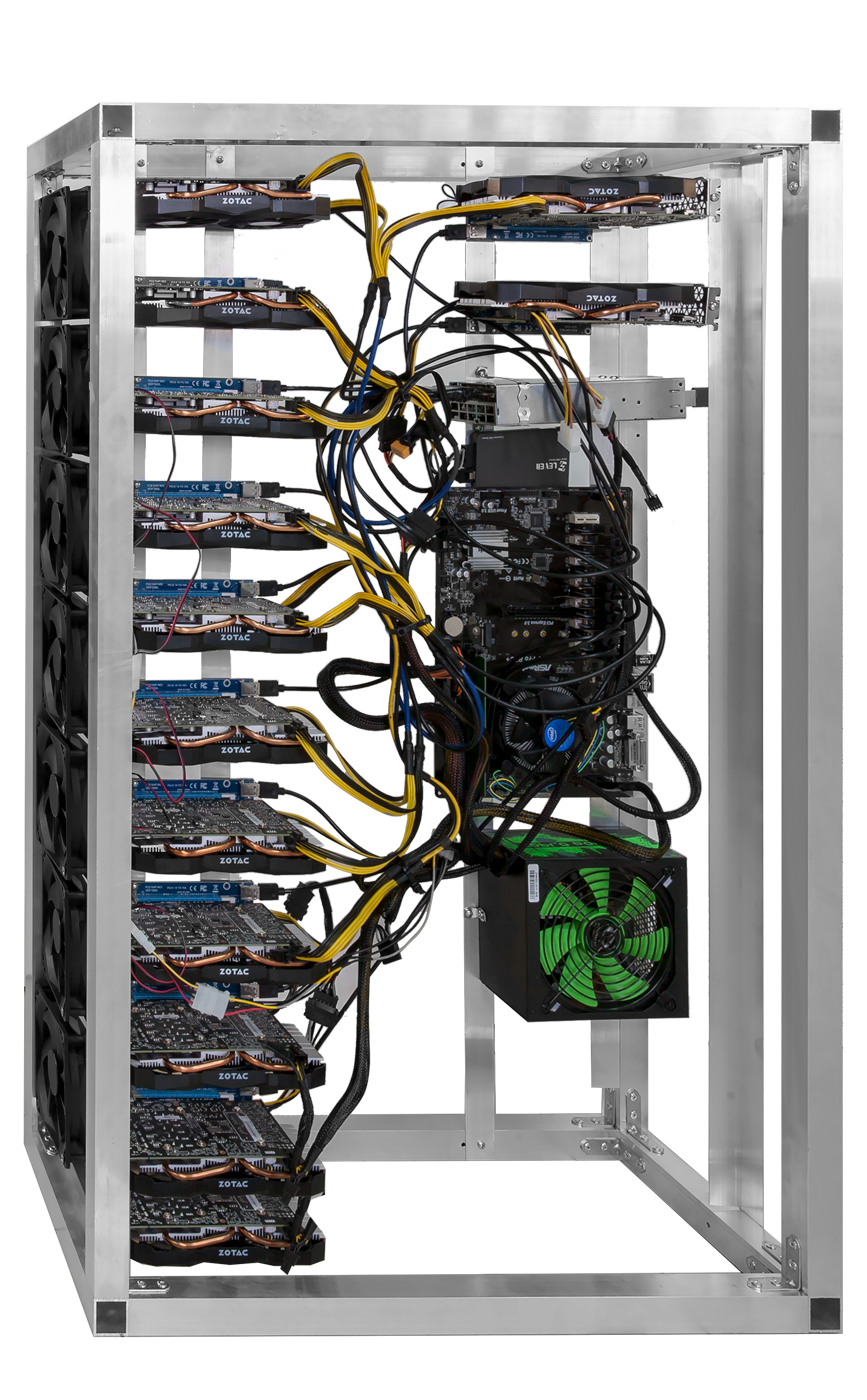
\includegraphics[width=.3\linewidth]{rig_mineracao.png}
    \end{center}
    \legend{Fonte: \url{https://mining.bg/13-gpu-mining-rig-nvidia-1060-3gb-8/}}
\end{figure}

A medida utilizada para apresentar o desempenho de um rig de mineração
é ``hashes por segundo'', representado por $\mathbf{h/s}$.
\emph{Hardware} e criptomoeda são fatores que variam a quantidade de
hashes por segundo.

\subsubsection{Pools de Mineração}

A mineração também pode ser feita em conjunto com os \emph{Pools} de
mineração. Onde um conjunto de mineradores trabalham em uma mesma
solução de um bloco. Quando solucionado, a recompensa é dividida
proporcionalmente; baseado na quantidade de trabalho feito, entre
todos os nodes da rede \cite{Weber2012}.

\emph{Pools} de mineração são vantajosos pelo fato de que independente
de quem solucione o bloco, a recompensa é dividida baseado no trabalho
do node. Diferente de quando se minera sozinho, onde a recompensa só é
ganha por uma pequena possibilidade.

\subsubsection{Monero}
% Descrever como o Monero surgiu e o que ele é
% Explicar como o monero tem um algoritmo de mineração que evita o
% uso por chips ASIC e FPGAs.
% TODO: Terminar esse parágrafo

O Monero usa um algoritmo de validação que dificulta a mineração por
chips especializados, como ASICs e FPGAs.  Tornando a mineração
somente lucrativa em CPUs ou GPUs \cite{Weber2012}. Os Rigs de
Mineração são valorizados dessa forma, já que o algoritmo de mineração
em uma GPU é muito mais eficiente que em um chip ASIC\@.

\subsubsection{Ethereum}
% Descrever como o Ethereum surgiu e o que ele é
% Explicar como o Ethereum também usa um algoritmo de mineração que
% evita o uso por chips ASIC e FPGAs.

\subsection{Sistema Operacionais Linux e Suas
Distribuições}\label{cap:sistemas-linux}

\subsubsection{Definição}

O Linux é um sistema operacional de código aberto, com mais de 100 mil
softwares livres desenvolvidos para rodarem nele, tornando as
possibilidades de que se encontre aplicações para criptomoedas muito
elevadas. Por ser muitas vezes grátis, seu custo geralmente se resume
no custo do meio, ou seja, no custo de um USB, DVD, CD ou plano de
rede \cite{Nunes2009}.

A atualização é feita de forma automática pela rede. Esta
característica é um requisito extremamente importante para a mineração
de criptomoedas, considerando que mudanças de implementação no sistema
são atualizadas automaticamente. No capítulo XXX apresentam-se
distribuições que são \emph{rolling release}, ou seja, que não
precisam de uma nova instalação para mudarem de versão
\cite{Nunes2009, ArchWiki2018a}.
% TODO: Referência cruzada aqui

\subsubsection{Distribuições Linux}

Uma distribuição Linux é uma variação do sistema operacional Linux
para um determinado contexto. O mapa de distribuições Linux contém
mais de $\mathbf{700}$ distribuições, organizadas pela data de criação
e hierarquia. Uma distribuição Linux pode ser baseada em outra, por
exemplo, o Linux Mint é baseado no Ubuntu, que baseia-se no Debian
\cite{Loli2017}.


\subsubsection{Meios de Instalação do Linux}

De modo resumido, a instalação do Linux pode ser feita de três
maneiras: (a) em modo convencional, onde é criada uma partição no
disco principal do computador e instalada; (b) de modo \emph{live},
onde no momento de \emph{boot} os arquivos do sistema são carregados
somente na memória RAM\@ e (c) de modo portátil, onde os arquivos do
sistema são instalados em uma mídia portátil \cite{Nunes2009}.

%O modo \emph{Live} permite a portabilidade, porém não permite a
%persistência de arquivos pessoais, geralmente este modo é utilizado
%para o usuário testar a distribuição antes da instalação. Para
%solucionar este problema, é possível, pela instalação portátil, manter
%um sistema que faz o \emph{boot} em uma mídia externa persistente.
%Após feita a configuração, o usuário tem um \emph{Desktop} pessoal
%portátil.

Uma distribuição Linux em modo Live cria um disco virtual na memória
RAM do computador em momento de boot, sem a persistência de arquivos.
Geralmente este modo é utilizado para o usuário testar a distribuição
antes de a instalar em um disco físico. Uma distribuição Linux em modo
portátil usa uma mídia portátil para persistir arquivos pessoais.

\begin{figure}[H]
    \caption{\label{fig:exemplo-distro}Uma distribuição Arch Linux
        instalada de maneira portátil. O \emph{boot} foi feito com um HD
    externo em um computador pessoal.}
    \begin{center}
        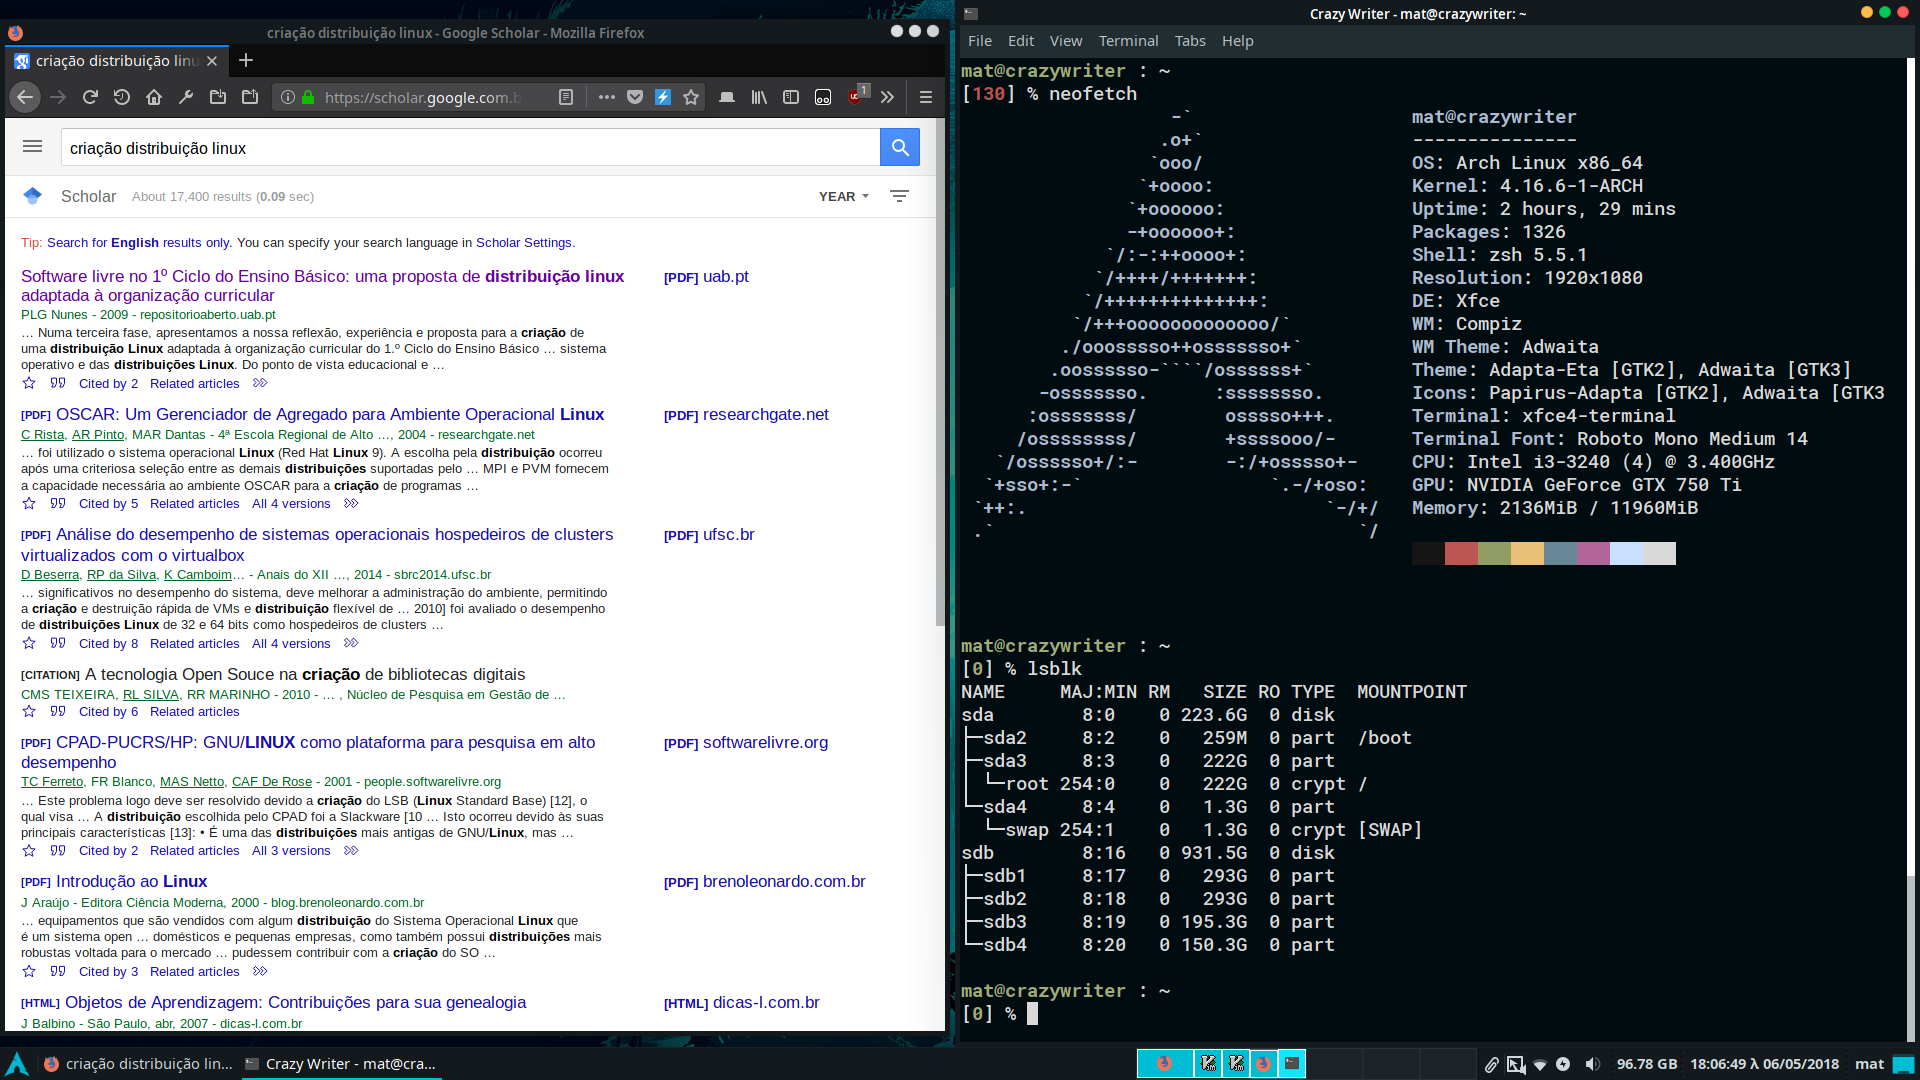
\includegraphics[width=\linewidth]{exemplo_arch.png}
    \end{center}
    \legend{Fonte: O Autor.}
\end{figure}

A Figura~\ref{fig:exemplo-distro} mostra a distribuição Arch Linux
instalada de modo portátil em um HD externo. Nessa figura são
apresentadas informações gerais de hardware/software e a
estrutura das partições, na qual \code{/dev/sda} representa o HD
externo e \code{/dev/sdb} representa o HD interno do Desktop.

\subsubsection{Criação de Uma Distribuição Linux}

% TODO: Ver a regra de citação direta na biblioteca
``A criação  de  distribuições  Linux pode fazer-se, a grosso modo,
através  de  dois processos distintos: criação de raiz ou criação a
partir de outra distribuição.'' \cite[p.  78]{Nunes2009}. A criação de
raiz demanda muito mais conhecimento técnico em programação de baixo
nível e sistemas operacionais, já que é preciso compilar o código
fonte.

Já a criação a partir de outra distribuição é feita com ``ferramentas
específicas, que  permitem adequar  a  nova  distribuição  aos
requisitos\ldots'' \cite[p. 78]{Nunes2009}, sendo um processo menos
trabalhoso. O \code{Archiso} é um exemplo de programa que cria
distribuições Linux customizadas a partir do Arch Linux. Dependendo da
ferramenta, nenhum conhecimento técnico avançado é necessário, já que
existem aplicações gráficas para criação de distribuições Linux, como
o Respin \cite{Respin2018} e o SuseStudio, que foi descontinuado.

Como dito anteriormente na Seção~\ref{cap:distribuicoes-linux}, uma
hierarquia é feita a partir de qual distribuição Linux é baseada em
qual.

\begin{figure}[H]
    \caption{\label{fig:hierarquia-arch}Gráfico da hierarquia do Arch
    Linux gerado com a ferramenta gnuclad \cite{Loli2017}.}
    \begin{center}
        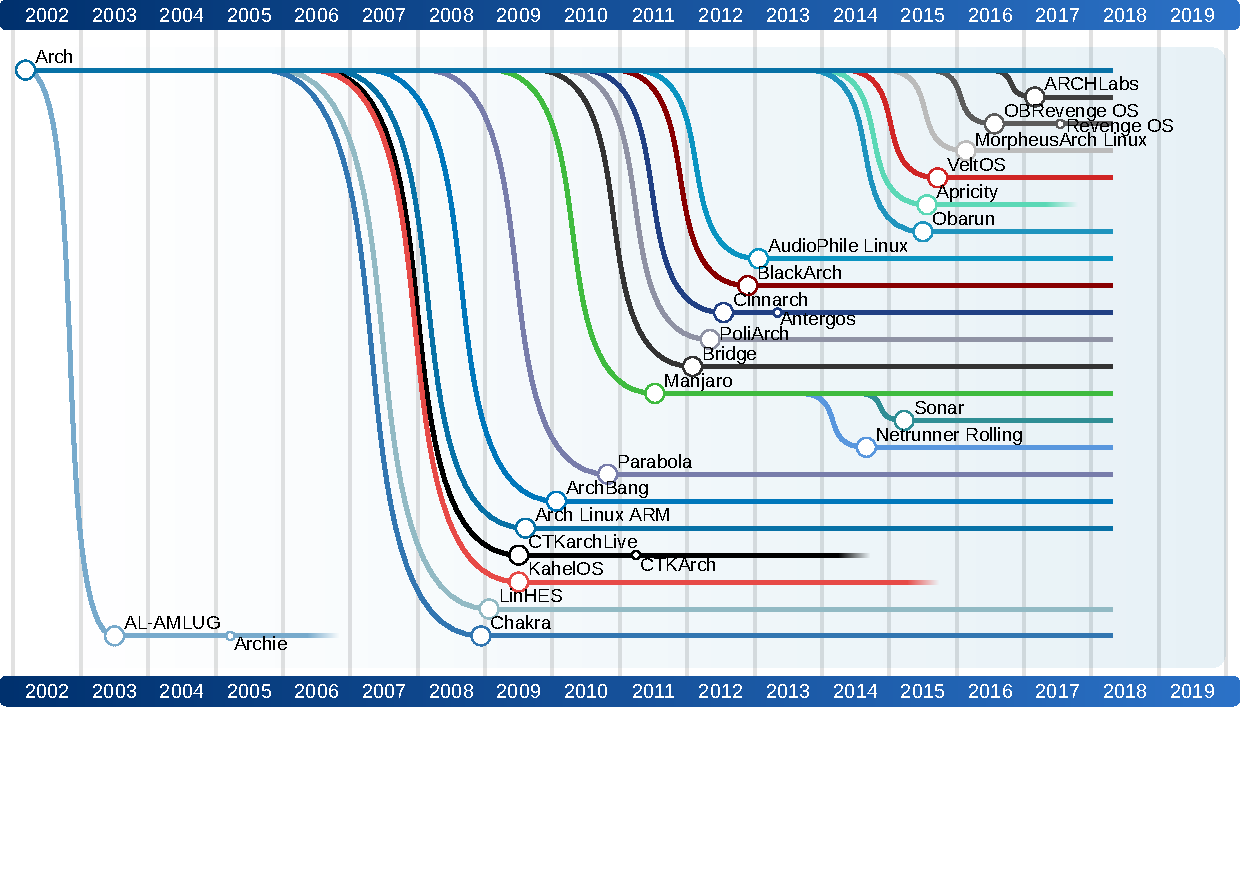
\includegraphics[width=.9\linewidth]{timeline_arch.pdf}
    \end{center}
    \legend{Fonte: O Autor.}
\end{figure}

Na Figura~\ref{fig:hierarquia-arch} é mostrada a hierarquia atual do
Arch Linux. Cada nó equivale a uma distribuição e a sua data de
criação é mostrada cronologicamente da esquerda para a direita.
Distribuições que são baseadas em outras são mostradas
hierarquicamente. Distribuições descontinuadas não continuam até o ano
2018. Mudanças de nomes no meio do projeto são mostradas por nós
menores.

Por exemplo, o Manjaro foi criada em $2011$ e é baseado no Arch. Já o
AL-AMLUG foi criado em $2003$ e mudou o nome para Archie que foi
descontinuado em $2005$.

\subsubsection{Debian}

O Debian é uma distribuição Linux que visa a estabilidade e código
aberto, com mais de $51.000$ pacotes pré compilados em seus
repositórios, ela se tornou uma distribuição muito difundida nos
últimos anos \cite{Debian2018}. Existem três versões do Debian,
(a) a \emph{stable} que tem uma ``vida útil'' de quatro anos e é a
mais destinada para usuários comuns, (b) a \emph{testing} que é
destinada para testes antes de virar uma \emph{stable} release e (c) a
\emph{unstable}, usada para o desenvolvimento de Debian.

Os gerenciadores de pacotes do Debian por linha de comando são o
\code{dpkg}, \code{apt} e \code{aptitude} \cite{Debian2016}. Para que
um pacote entre nos repositórios oficiais do Debian, é necessário que
ele siga regras rigorosas de software livre. Repositórios não oficiais
devem ser adicionados manualmente pelo usuário.

\subsubsection{Ubuntu}

Como o Debian não é muito convidativo para usuários sem um
conhecimento técnico moderado, em $2004$, o Ubuntu surgiu como uma
distribuição construída com foco em usabilidade. Sua versão Desktop
possui vários pacotes já instalados para um uso genérico do dia a dia,
como softwares para edição de texto, reprodutores de mídia e
interfaces gráficas \cite{UbuntuFundation2018}.

Por ser uma distribuição baseada no Debian, existem semelhanças entre
as duas. Sua versão estável, ou \emph{LTS release}, tem suporte por
cinco anos \cite{UbuntuWiki2017}. Variações como o Ubuntu Server são
destinadas a servidores e não tem uma interface gráfica. Outras
variações criadas pela comunidade, como o Kubuntu e Xubuntu, somente
apresentam interfaces gráficas diferentes.

Os gerenciadores de pacotes do Ubuntu são iguais ao Debian e a
utilização de um repositório não oficial exige que o usuário o
adicione manualmente \cite{UbuntuWiki2018}.

\subsubsection{Fedora}

Tendo suas raízes no Red Hat, o Fedora é uma distribuição criada para
facilitar a vida do usuário. Suas duas versões, (a) a
\emph{Workstation} destinada a Desktops e (b) a \emph{Server}
destinada a servidores possuem interfaces gráficas
\cite{FedoraProject2018}. As versões do Fedora focam a estabilidade e
são atualizadas em média a cada 13 meses \cite{FedoraProject2018a}.

Seu gerenciador de pacotes é o \code{rpm}, o mesmo do Red Hat. Como no
Debian e Ubuntu, repositórios não oficiais devem ser adicionados
manualmente \cite{FedoraProject2018b}.

\subsubsection{Arch}

O Arch Linux é uma distribuição que visa a versatilidade e
estabilidade. Destinada a usuários mais experientes, no momento de
instalação, é mostrada uma linha de comando para que o usuário escolha
quais pacotes vão ser instalados. Seu modelo de atualização é
\emph{rolling release}, ou seja, os pacotes da distribuição são
atualizados incrementalmente, em vez de existir um número ou tipo fixo
de versão \cite{ArchWiki2018a}. É uma distribuição estável, porem é
necessário verificar os canais de notícias do Arch Linux para
eventuais intervenções manuais no momento de atualização
\cite{ArchWiki2018c}.

O que distingue o Arch de outras distribuições é o seu gerenciador de
pacotes \code{pacman} que usa o \code{PKGBUILD}, um modelo de criação
de pacotes para a distribuição, que permite que até programas que só
funcionam no Windows tenham pacotes no repositório da comunidade. Este
repositório da comunidade se chama \code{AUR} e qualquer usuário do
Arch Linux pode adicionar um novo pacote no repositório, desde que
regras básicas sejam seguidas \cite{ArchWiki2018d}.

\begin{figure}[H]
    \caption{\label{fig:exemplo-aur}O programa Algodoo, um simulador
    de física que só tem uma versão oficial no Windows.}
    \begin{center}
        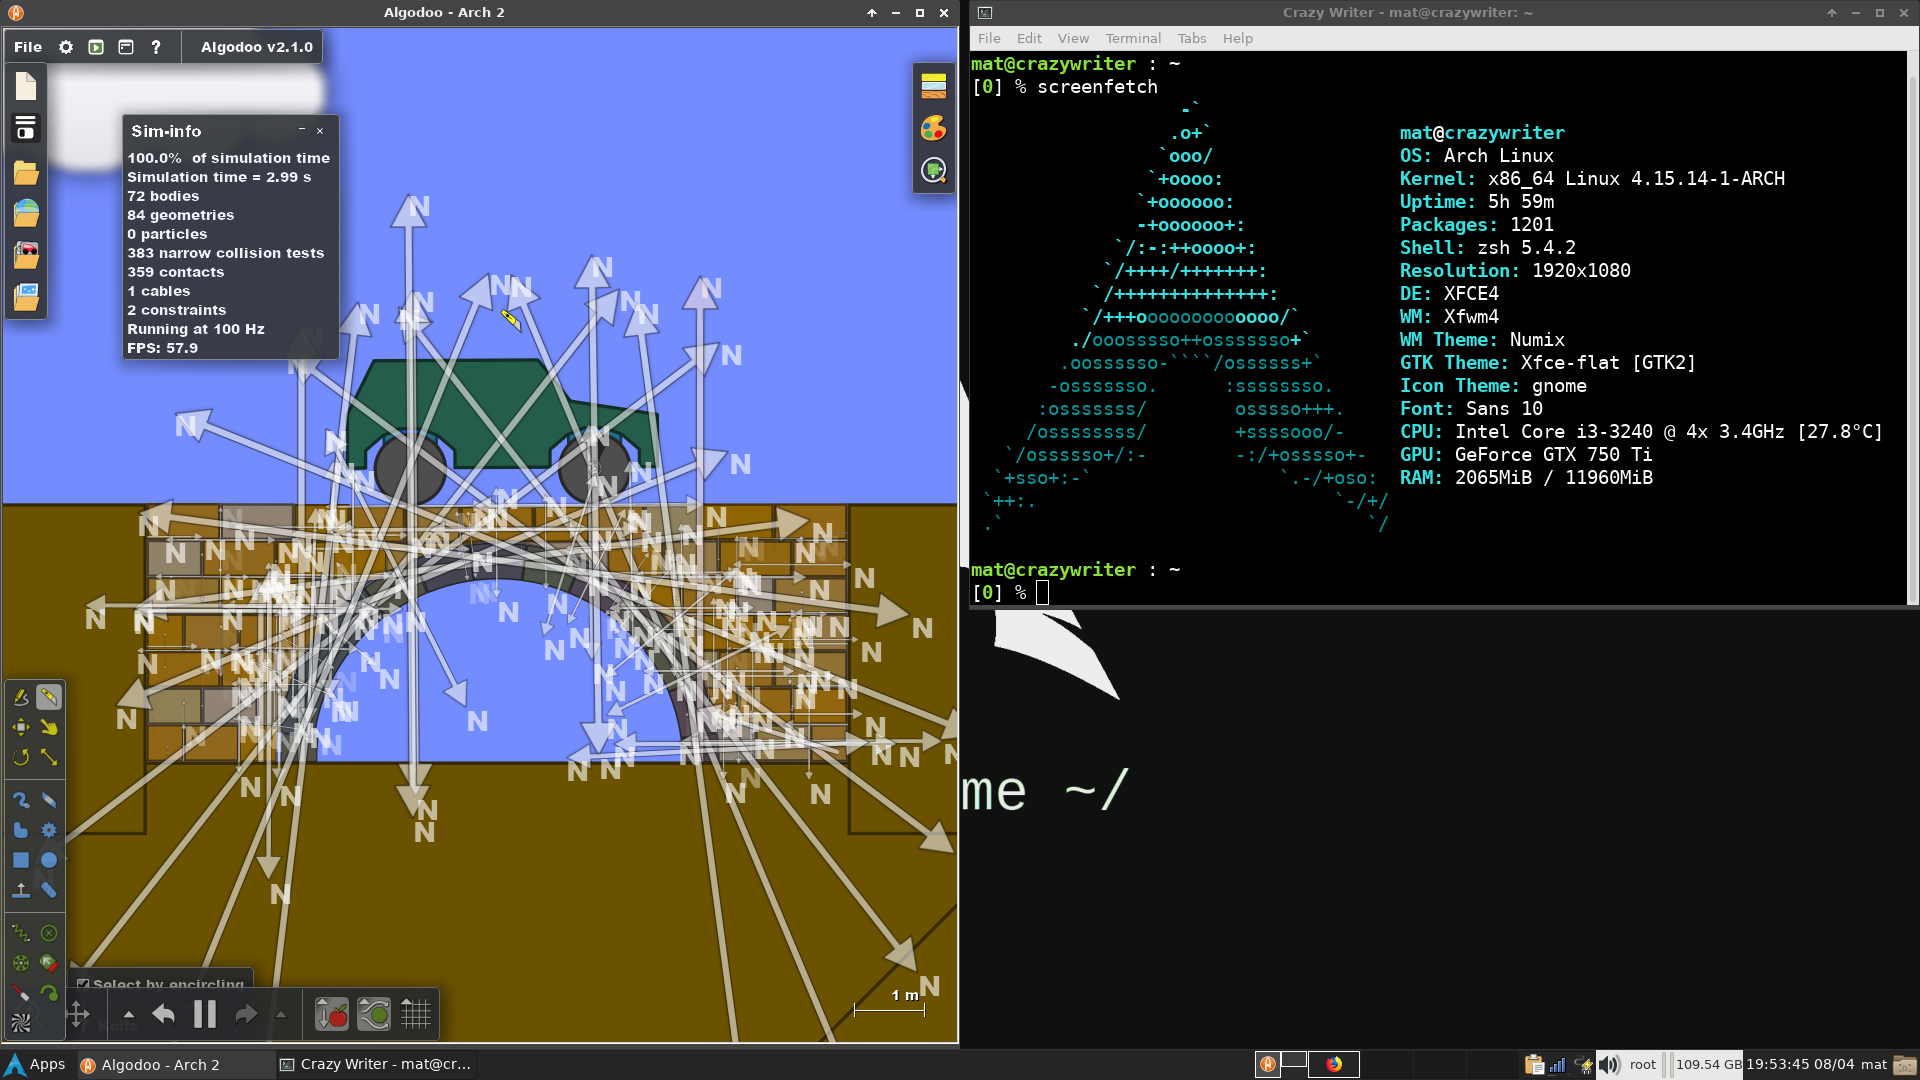
\includegraphics[width=\linewidth]{exemplo_aur.png}
    \end{center}
    \legend{Fonte: O Autor.
    \url{https://github.com/MatMercer/aur-algodoo}}
\end{figure}

A Figura~\ref{fig:exemplo-aur} mostra o pacote \code{algodoo-wine},
disponível no \code{AUR}. A instalação do programa é feita utilizando
a ferramenta \code{innoextract} para a extração dos binários do
instalador Windows para serem executados com o programa \code{WINE}.

\subsubsection{Gentoo}

Todas as distribuições discutidas anteriormente são binárias, isto
quer dizer que o Kernel, o programa que faz a interface entre o
hardware e software, já vem compilado. O Gentoo é baseado no FreeBSD e
possui várias semelhanças com o Arch Linux \cite{GentooFundation2018}.
Por exemplo, seu modelo de atualização também é \emph{rolling release}
e seu principal foco é a customização. No quesito estabilidade é que
surgem as maiores diferenças.

O Portage é seu gerenciador de pacotes, e a maioria desses pacotes
devem ser compilados no momento de instalação \cite{GentooWiki2018}.
Como o Kernel também é compilado, podem surgir problemas como a falta
de bibliotecas e/ou bugs no código dos pacotes. Devido a esse fato,
sua estabilidade é comprometida e o usuário deve ter um conhecimento
técnico maior, além de ter uma cautela maior no momento de instalação.

O Gentoo, com o passar dos anos, virou a referência de uma
distribuição para quem quer aprender mais sobre Unix, pois seu modo de
instalação exige um estudo mais aprofundado. Porém, não tão
aprofundado outras distribuições, como o Linux From Scratch.

\subsubsection{Características Relevantes em Distribuições Linux Para Mine-
ração de criptomoedas}

São características importantes de uma distribuição: (a) Ela deve ser
capaz de minerar moedas que são possíveis de serem mineradas
lucrativamente em computadores domésticos e (b) deve suportar rigs de
mineração por meio de drivers. No quesito tamanho, sua ISO deve ter no
máximo 4GB\@.

No quesito gerenciador de pacotes, (a) devem ser suficientemente
estáveis, (b) instalação e atualização deve ser simples, (c) deve
possuir a disponibilidade de pacotes com código fechado já que drivers
de NVidia não são open-source, (d) a quantidade de pacotes deve ser
extensa e (e) as versões do pacote não devem ser muito antigas.

A Tabela~\ref{table:quadro-comparativo} mostra o comparativo entres as
distribuições discutidas no Capítulo~\ref{cap:sistemas-linux}.

\subsubsection{Quadro Comparativo Entre Distribuições Linux Para a
Proposta do Trabalho}

\begin{table}[H]
    \centering
    \caption{\label{table:quadro-comparativo}Quadro Comparativo Entre
    Distribuições Linux}
    \makebox[\textwidth]{%
        \begin{tabularx}{1\textwidth}{>{\raggedright}p{3cm}cccccc}
            \toprule
            \multicolumn{1}{l}{\bfseries Distribuição} &
            \multicolumn{1}{c}{Debian} &
            \multicolumn{1}{c}{Ubuntu} &
            \multicolumn{1}{c}{Fedora} &
            \multicolumn{1}{c}{Arch} &
            \multicolumn{1}{c}{Gentoo} \\
            \midrule

            \textbf{Tamanho da ISO}              & 600MB ou 4.7GB & 1.5GB & 1.5GB & 600MB & 300MB ou 2GB \\
            \midrule
            \textbf{Taxa de Atualização}         & Baixa & Média & Alta & Alta & Alta \\
            \midrule
            \textbf{Disponibilidade de Pacotes}  & Média & Alta & Alta & Alta & Alta \\
            \midrule
            \textbf{Pacotes de Código Fechado}   & Sim & Sim & Não & Sim & Parcialmente \\

            \toprule
        \end{tabularx}
    }
\end{table}

% ----------------------------------------------------------
% Referências bibliográficas (nome do arquivo de referencias, sem o
% ".bib"
% ----------------------------------------------------------
\pagebreak \bibliography{referencias}

\end{document}
